\documentclass[tikz,border=2]{standalone}
%tags: arrow for tikzimg figure neural neuralNetwork graph network forLoop
%macro
\usepackage{amssymb}
\usetikzlibrary{shadows,arrows,shapes,positioning,calc,backgrounds,fit}
\begin{document}
%%%%%%%%%%%%%%%%%%%%%%%%%%%%%%%%%%%%%%%
% colors
\definecolor{myBlue}{HTML}{0060AD}
\definecolor{myRed}{HTML}{DD181F}
%%%%%%%%%%%%%%%%%%%%%%%%%%%%%%%%%%%%%%%

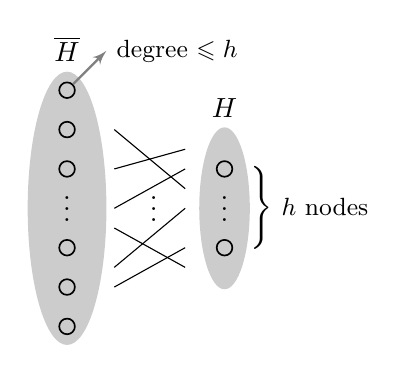
\begin{tikzpicture}
[scale=1,transform shape,
node distance=1cm,
%
vertex/.style={shape=circle,draw=black,inner sep=2pt,semithick},
seed/.style={vertex,fill=red},
infected/.style={vertex,fill=brown},
%
every edge/.style={draw},
dedge/.style={gray,>=latex', shorten >=.0pt, shorten <=.0pt, thick}]
%
% H
\foreach \x in {3,...,3}
\node (b\x) [vertex] at (2,.5*\x) {};
\node at (2,2.1) {$\vdots$};
\foreach \x in {5,...,5}
\node (b\x) [vertex] at (2,.5*\x) {};
\begin{pgfonlayer}{background}
\node[fill=black!20,ellipse,fit=(b3)(b5),label=above:${H}$]{};
\end{pgfonlayer}
% complement H
\foreach \x in {1,...,3}
\node (a\x) [vertex] at (0,.5*\x) {};
\node at (0,2.1) {$\vdots$};
\foreach \x in {5,...,7}
\node (a\x) [vertex] at (0,.5*\x) {};
\begin{pgfonlayer}{background}
\node[fill=black!20,ellipse,minimum width=1cm,fit=(a2)(a6),label=above:$\overline{H}$]{};
\end{pgfonlayer}
% edges
\path
(.6,1.75) edge (1.5,1.25)
(.6,1) edge (1.5,1.5)
(.6,1.25) edge (1.5,2)
(.6,2) edge (1.5,2.5)
(.6,2.5) edge (1.5,2.75)
(.6,3) edge (1.5,2.25);
\node at (1.1,2.1) {$\vdots$};
%
\draw[->,dedge] (a7) -- ++(.5,.5) node [right,black] {\small degree $\leqslant h$};
\node [right] at (2.2,2) {$\Bigg\}$ {\small $h$ nodes}};
\end{tikzpicture}
{}
\end{document}
